\section{Conceptos previos}
En este apartado se describe la arquitectura de VMware Cloud Foundation y como estructura sus componentes\footnote{Se describen solo aquellos componentes que se utilizarán en el despliegue de Cloud Foundation.} internamente.

%%%%%%%%%%%%%%%%%%%%%%%%%%%%%%
\iffalse
En este apartado se explican aquellos conceptos de VMware Cloud Foundation necesarios para entender su funcionamiento, configuración y requisitos de la infraestructura previos al despliegue del servicio.
\fi
%%%%%%%%%%%%%%%%%%%%%%%%%%%%%%%%


%% Workload Ddomains %&%&%%%%
%%%%%%%%%%%%%%%%%%%%%%%%%%%%
\subsection{Workload Domain}
Un \textit{workload domain} consiste en una instancia lógica de un SDDC que abarca todos o parte de los recursos de uno o más clusters, cuya función es aislar el flujo de trabajo de un usuario, aplicación o un determinado tipo de tareas. Cada \textit{workload domain} se extiende sobre varios hosts y contiene su propia instancia de vCenter Server, vSAN y NSX, lo cual permite establecer políticas de control únicas para todos los \textit{workload domains} y específicas para cada uno de ellos a la vez que se simplifica la complejidad de la infraestructura. Existen \underline{tres tipos} de \textit{workload domains} que permiten aislar las tareas de gestión de la infraestructura del resto de flujos de trabajo. 

%% MANAGEMENT DOMAIN
\subsubsection{Management Domain}
\label{subsubsec:domainManagement}
Este \textit{workload domain} se crea y configura automáticamente durante el proceso de despliegue de una instancia de VMware Cloud Foundation. Su función es gestión de todos los componentes de VMware Cloud Foundation, de toda la infraestructura y del resto de \textit{workload domains} existentes en el entorno a tráves de políticas establecidas desde un único punto. Los componentes dedicados a este \textit{workload domain} son SDDC Manager, vCenter Server, una instancia de NSX Manager, tres instancias de NSX Controller, dos instancias de Platform Services Controller y tres instancias de vRealize Log Insight \cite{sddcComponents} [Fig. \ref{fig:componentsMNGDomain}].\\
Cuando se \underline{despliega \textit{management domain} se crean y configuran} de forma automatizada por SDDC Manager las siguientes máquinas virtuales (VM) de cada componente de Cloud Foundation\footnote{Las características de cada máquina virtual se refieren a los requisitos mínimos}:
\begin{itemize}
    \item Una VM de \textbf{SDDC Manager}: 4 vCPU, 16 GB de memoria, 800 GB de almacenamiento.
    \item Una VM de \textbf{vCenter Server}: 4 vCPU, 16 GB de memoria, 290 GB de almacenamiento.
    \item Dos instancias de \textbf{Platform Services Controller} (cada una): 2 vCPU, 4 GB de memoria, 60 GB de almacenamiento.
    \item Una VM de \textbf{NSX Manager}: 4 vCPU, 16 GB de memoria, 60 GB de almacenamiento.
    \item Tres VM de \textbf{NSX Controller} (cada una): 4 vCPU, 4 GB de memoria, 28 GB de almacenamiento.
    \item Tres VM de \textbf{vRealize Log Insight}: 4 vCPU, 8 GB de memoria, 250 GB de almacenamiento.
\end{itemize}

Para desplegar un \textit{management domain} se requieren las siguientes \underline{capacidades mínimas} en la infraestructura \cite{WDminRequierements}:
\begin{itemize}
    \item \textbf{Hosts}: 4
    \item \textbf{CPU} por host: Dual-socket con 8 cores por socket, en sistemas All-Flash.
    \item \textbf{Memoria} total: 192 GB
    \item \textbf{Almacenamiento} por host: 16 GB para el dispositivo de arranque, un NVMe o SSD para la capa de caché, dos SSD o HDD para la capa de capacidad\footnote{En total se requieren 800 GB para este \textit{workload domain}.}.
    \item \textbf{NICs} por host: Dos NICs de al menos 10 GbE y, opcionalmente un NIC 1GbE BMC.
\end{itemize}

\begin{figure}[h!]
  \centering
  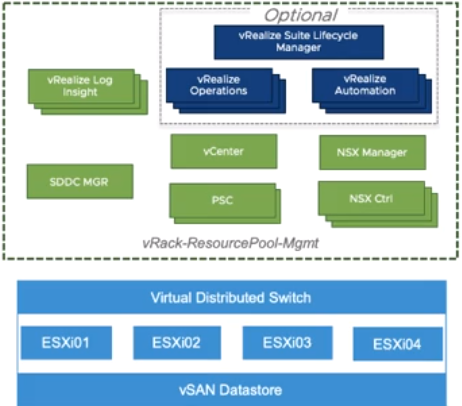
\includegraphics[width=0.8\textwidth]{imaxes/conceptosPrevios/componentsMANAGEDomain.png}
  \caption{Componentes de \textit{management domain}}
  \label{fig:componentsMNGDomain}
\end{figure}
\FloatBarrier 


%% VIRTUAL INF. DOMAIN
\begin{subsubsection}{Virtual Infrastructure Domain (VI) y Virtual Desktop Infrastructure Domain (VDI)}
\label{subsubsec:domainVI}
Este tipo de \textit{workload domain} se crea manualmente y bajo demanda desde \textit{management domain} para dar servicio a las necesidades de cada usuario o para crear diferentes entornos con finalidades distintas. Su configuración de hardware y lógica se especifican durante su proceso de creación, permitiendo indicar la cantidad de hosts, cantidad de almacenamiento, configuración de la red y políticas de rendimiento y disponibilidad, todo para satisfacer las necesidades del tipo de tareas para las que se crea. El acceso a un \textit{VI domain} se realiza a través de vSphere Client donde el administrador puede gestionar todos los recursos asociados con ese \textit{workload domain}. Cada \textit{virtual infrastructure domain} cuenta con sus propios vCenter Server y un NSX Manager dedicados, que se ejecutan desde el \textit{management domain} de la infraestructura, y \textit{datastore} vSAN dedicado. La diferencia entre un \textit{virtual infrastructure domain} y \textit{virtual desktop infrastructure domain} es que el segundo incorpora el producto VMware Horizon View que, resumiendo, permite desplegar escritorios virtuales. Con cada nuevo \textit{virtual infrastructure domain} se crea un nuevo cluster vSphere en la infraestructura que agrupa todos los recursos que tiene asignados.\\
Cuando se \underline{despliega un \textit{virtual infrastructure domain} se crean y configuran} de forma automatizada por el componente SDDC Manager las siguientes máquinas virtuales (VM) de cada componente de VMware Cloud Foundation\footnote{Las características de cada máquina virtual se refieren a los requisitos mínimos} \cite{sddcComponents} [Fig. \ref{fig:compoVIdomain}]:
\begin{itemize}
    \item Una VM de \textbf{vCenter Server} en Management Domain: 8 vCPU, 24 GB de memoria, 500 GB de almacenamiento.
    \item Una VM de \textbf{NSX Manager} en Management Domain: 4 vCPU, 16 GB de memoria, 60 GB de almacenamiento.
    \item Tres VM de \textbf{NSX Controller} en el VI Domain creado (cada una):  4 vCPU, 4 GB de memoria, 28 GB de almacenamiento.
\end{itemize}

Por cada \textit{virtual infraestructure domain} que se despliega en la infraestructura, se requieren las siguientes capacidades mínimas\cite{WDminRequierements}:
\begin{itemize}
    \item \textbf{Hosts}: 3
    \item \textbf{CPU}, \textbf{Memoria} y \textbf{Almacenamiento}: depende de los requisitos de las tareas que se vayan a desarrollar en este \textit{workload domain}.
    \item \textbf{NICs} por servidor: Dos NICs de al menos 10 GbE y, opcionalmente un NIC 1 GbE BMC.
\end{itemize}


\end{subsubsection}

\begin{figure}[h!]
  \centering
  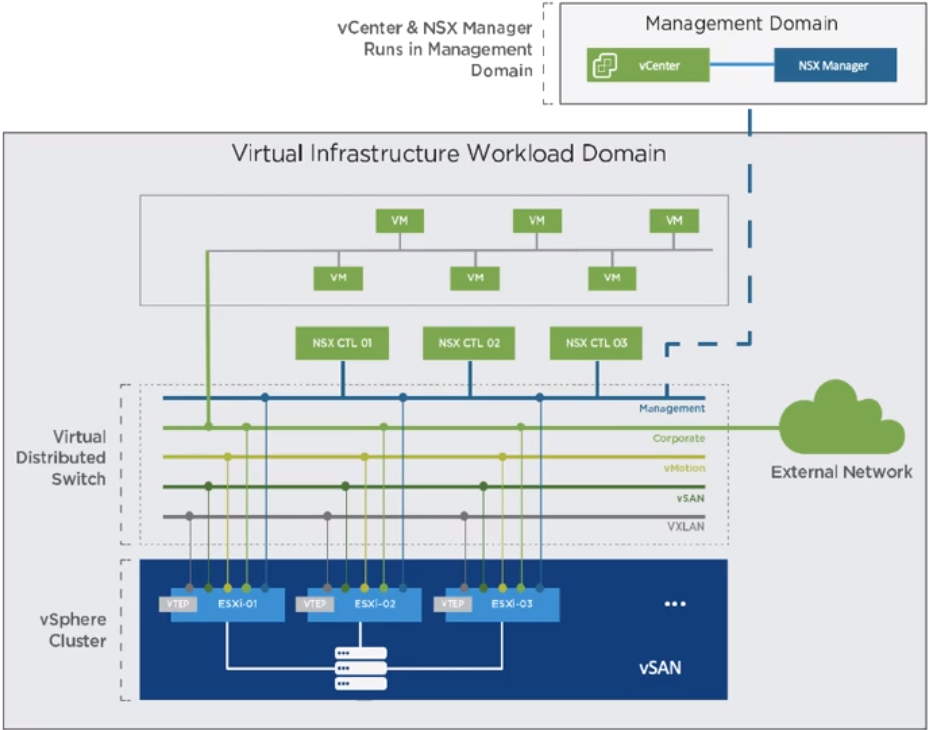
\includegraphics[width=1\textwidth]{imaxes/conceptosPrevios/networkArcVIDomain.png}
  \caption{Componentes de \textit{virtual infrastructure domain}.}
  \label{fig:compoVIdomain}
\end{figure}
\FloatBarrier

%&%%%%%%%%%%%%%%%%%%%%%%%%%%%%%%%%%%%%%%%%%%%%%%%%%%%%%%%%
%% ARQUITECTURA



\subsection{Arquitectura}
La arquitectura de VMware Cloud Foundation tiene dos posibles modelos de despliegue dependiendo del número de hosts sobre los que se despliega VMware Cloud Foundation.

%% ESTANDAR
\subsubsection{Modelo estándar}
Este modelo está pensado para desplegar VMware Cloud Foundation en entornos de tamaño medio/grande con un mínimo de siete hosts. Está formado por un \textit{management domain} que se despliega en cuatro de los hosts y contiene todos los componentes de gestión de toda la infraestructura, desde este \textit{workload domain} se administra la infraestructura del SDDC y cada \textit{virtual infrastructure domain} existente. Además, este modelo contiene al menos un \textit{virtual infrastructure domain}, creado bajo demanda y con capacidades establecidas según su finalidad que posteriormente se pueden pueden modificar, se despliega sobre al menos tres hosts. Cada \textit{virtual infrastructure domain} requiere tres hosts adicionales, es decir, un host solo puede pertenecer a un único \textit{workload domain}. El máximo número de \textit{virtual infrastructure domains} que se pueden desplegar en una instacia de VMware Cloud Foundation es 14.

\begin{figure}[h!]
  \centering
  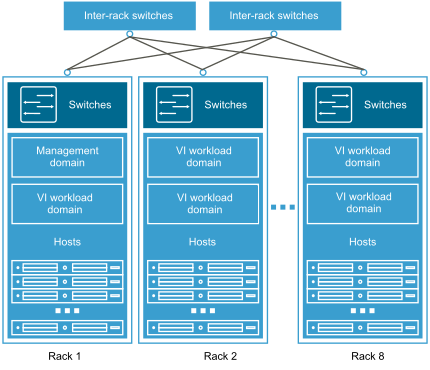
\includegraphics[width=0.75\textwidth]{imaxes/conceptosPrevios/arquitect_standarCF.png}
  \caption{Esquema del modelo de arquitectura estándar.}
  \label{fig:modelostandard}
\end{figure}

\begin{figure}[h!]
  \centering
  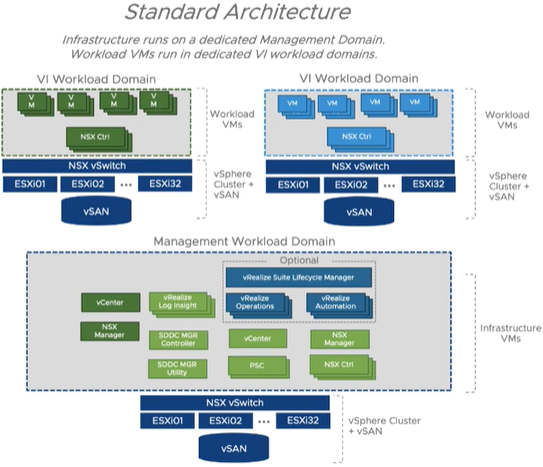
\includegraphics[width=0.85\textwidth]{imaxes/conceptosPrevios/standardArch.png}
  \caption{Estructura de los componentes en una arquitectura estándar.}
  \label{fig:standardarch}
\end{figure}
\FloatBarrier
%%%%%%%%%%%%%%%%%%%%%
%%  CONSOLIDADO
\subsubsection{Modelo consolidado}
Este modelo está pensado para desplegar VMware Cloud Foundation en entornos de tamaño pequeño, normalmente cuando hay menos de siete hosts, aunque se puede también se puede utilizar sobre entornos más grandes de hasta 64 hosts. En este modelo los flujos de trabajo que corresponden al \textit{virtual infrastructure domain} y al \textit{management domain} en el despliegue estándar, están colocados dentro de un mismo \textit{workload domain} en un único cluster pero aislados gracias a que cada uno se coloca dentro de un \textit{resource pool}, es decir, solo existe un cluster con varios \textit{resource pool}. Un \textit{resource pool} es una carcaterística de VMware vSphere que permite abstraer un conjunto de recursos de un cluster estableciendo unos límites de capacidad que puede usar \cite{resourcePool}. Este modelo se puede convertir en un modelo estándar creando un \textit{virtual infrastructure domain}.[Fig. \ref{fig:modeloconsolidated}].

\begin{figure}[h!]
  \centering
  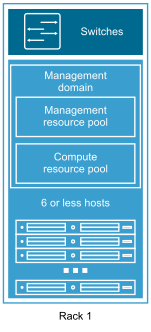
\includegraphics[width=0.25\textwidth]{imaxes/conceptosPrevios/modelConsolidated.png}
  \caption{Esquema del modelo de arquitectura consolidado.}
  \label{fig:modeloconsolidated}
\end{figure}

\begin{figure}[h!]
  \centering
  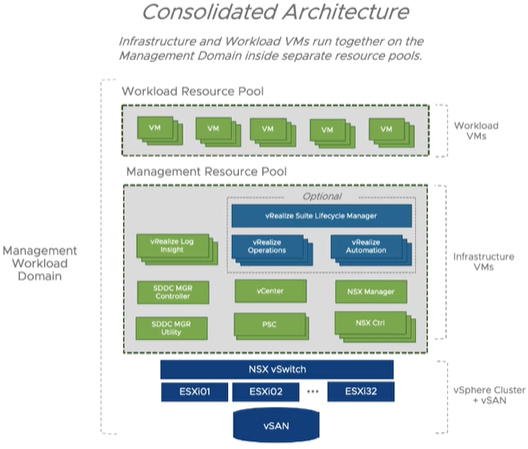
\includegraphics[width=0.85\textwidth]{imaxes/conceptosPrevios/consolidatedArch.png}
  \caption{Estructura de los componentes de una arquitectura consolidado.}
  \label{fig:consolidatedArch}
\end{figure}
\FloatBarrier


\section{Requisitos y diseño de la infraestructura y arquitectura}

Teniendo en cuenta las capacidades físicas de la infraestructura, se ha elegido el modelo consolidado para el despliegue de VMware Cloud Foundation sobre la infraestructura. 
La principal razón por las que se escoge este modelo es por el número de hosts ESXi.\\
En los siguientes apartados se describen la arquitectura que se genera y la infraestructura requerida en cada capa.

%%%% DISEÑO ARQUI. FÍSICA %%%%%
\begin{subsection}{Arquitectura e Infraestructura Físicas \cite{CFfisInfraestuctura}}
En este apartado se describen las principales características que tiene el entorno físico de un SDDC construído con VMware Cloud Foundation.

\subsubsection{Clusters, zonas de disponibilidad y regiones}
Un SDDC puede estar formado por uno o más clusters de distintos tipos. En el  \underline{modelo consolidado} la infraestructura está formada por un único cluster que incluye los servicios de gestión de VMware Cloud Foundation VMware vCenter Server, vSphere Update Manager, VMware NSX Manager, VMware NSX Controller y VMware vRealize Log Insight, los servicios de red necesarios para establecer conectividad en el entorno y las máquinas virtuales que los usuarios crean cuando aprovisionan sus recursos. Se aplican las mismas políticas de alta disponibilidad y gestión del ciclo de vida al flujo de trabajo de gestión del SDDC y al flujo de trabajo del usuario. En el \underline{modelo estándar} los distintos \textit{workload domain} se dividen en clusters que pueden ser de tres tipos:
    \begin{itemize}
        \item \textbf{Management Cluster}: se crea durante el despliegue de VMware Cloud Foundation y contiene el \textit{management domain}, desde aquí se gestiona el SDDC. Contiene los servicios de gestión mecionados anteriormente.
        \item \textbf{Shared Edge and Compute Cluster}: es el primer cluster que se crea dentro de un \textit{virtual infrastructure domain} ya que puede haber más de un cluster. Este cluster contiene los servicios de red NSX del \textit{workload domain} y también puede contener el flujo de trabajo de los usuarios.
        \item \textbf{Compute Cluster}: cluster adicional que se crea dentro de un \textit{virtual infraestructure domain}. Contiene el flujo de trabajo de los usuarios.
    \end{itemize}
Un SDDC puede estar distribuído en una o más \textit{Availability Zone} (AZ). Estas son zonas aisladas con infraestructuras independientes que evitan la propagación de fallos de hosts individuales a través de toda la infraestructura, cuantas más \textit{AZ} existan mayor disponibilidad tendrá el servicio. La latencia entre dos \textit{AZ} debe ser de 5 ms como máximo y la conexión de al menos 10 Gbit. Una \textit{Region} agrupa una o más \textit{AZ}s, con esto se da solución a la recuperación del servicio ante desastres. La latencia entre dos \textit{Region}s debe ser de 100 ms como máximo. El \underline{modelo consolidado} solo da soporte a una \textit{Region} con una \textit{AZ}, mientras que el \underline{modelo estándar} puede soportar múltiples \textit{Region}s con múltiples \textit{AZ}s.

%%%%%%%%%%%%%%%%%%%%%%%%%%%%%%%%%%%%%%%%%%%%
%%%%%%%%%%%%%%%%%%%%%%%%%%%%%%%%%%%%%%%%%%%%
%%%%%%%%%%%%%%%%%%%%%%%%%%%%%%%%%%%%%%%%%%%%
\iffalse
Un SDDC puede estar \underline{formado por múltiples clusters} que pueden ser de diferentes tipos con diferentes propósitos. Un cluster puede ocupar uno o más \textit{racks} dependiendo del nivel de escalabilidad que se requiera. Según su función, cada \textit{workload domain} se puede colocar en un cluster diferente para gestionar la alta disponibilidad y el ciclo de vida según sus necesidades. Un \underline{cluster puede ser de varios tipos}:
\begin{itemize}
    \item \textbf{Management Cluster}: Es aquel que contiene el \textit{management domain}, por lo tanto contiene las máquinas virtuales de los componentes que gestionan el SDDC. A este cluster solo deben acceder los administradores de la infraestructura.
    \item \textbf{Shared Edge y Compute Cluster}: contiene el \textit{virtual infrastructure domain} con las máquinas virtuales de los usuarios y, además, incorpora servicios de NSX necesarios para comunicarse con redes externas y con otros \textit{workload domains}.
    \item \textbf{Compute Cluster}: solo contiene el \textit{virtual infrastructure domain} con las máquinas virtuales de los usuarios.
    \item \textbf{External Storage}: se centra en proveer almacenamiento de tipo NFS, iSCSI o Fiber Channel.
\end{itemize}

Un SDDC puede estar distribuído en una o más \underline{zonas de disponibilidad}. Estas son zonas aisladas que evitan la propagación de fallos de hosts individuales a través de toda la infraestructura, así, se puede entregar mayor disponibilidad de los recursos y servicios. A su vez, varias \underline{zonas de disponibilidad} se pueden agrupar en una \underline{región}, estos entornos separados por grandes distancias que permiten tener recuperación ante desastres [Fig. \ref{fig:AVRegiones}].\\

\begin{figure}[h!]
  \centering
  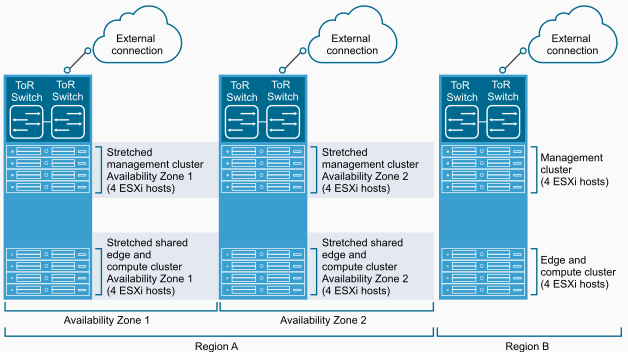
\includegraphics[width=0.95\textwidth]{imaxes/conceptosPrevios/zonasDispRegiones.png}
  \caption{Una región contiene al menos una zona de disponibilidad.}
  \label{fig:AVRegiones}
\end{figure}
\fi
%%%%%%%%%%%%%%%%%%%%%%%%%%%%%%%%%%%%%%%%%%%%%
%%%%%%%%%%%%%%%%%%%%%%%%%%%%%%%%%%%%%%%%%%%%%
%%%%%%%%%%%%%%%%%%%%%%%%%%%%%%%%%%%%%%%%%%%%%

\FloatBarrier

\subsubsection{Red física}
La topología de red en la capa física del SDDC de VMware Cloud Foundation se puede implementar mediante servicios de \underline{transporte} en la capa 2 o en la capa 3. El \underline{diseño en la capa 2} implica que la topología de la red incluya los dispositivos de capa 2 (\textit{Top of Rack Switches}) y los dispositivos de la capa 3 (routers, switches) [Fig. \ref{fig:transportlayer2}], por lo tanto las VLANs que se definan se deben implementar en la capa 2 y en la capa 3. Esto puede provocar problemas al aumentar el tamaño de la red ya que el número de VLANs disponible es más limitado, y problemas de compatibilidad ya que es posible que los dispositivos físicos tengan que ser del mismo proveedor. El \underline{diseño en la capa 3} implica que la topología de la red solo incluye a los dispositivos de capa 3 [Fig. \ref{fig:transportlayer3}]. Esto permite limitar la definición de VLANs a esa capa y el uso de enrutamiento dinámico con protocolos OSPF o BGP entre la capa 2 y 3. Así se consigue una mayor libertad a la hora de seleccionar los dispositivos físicos de red y que su configuración es más sencilla.
\begin{figure}[h!]
  \centering
  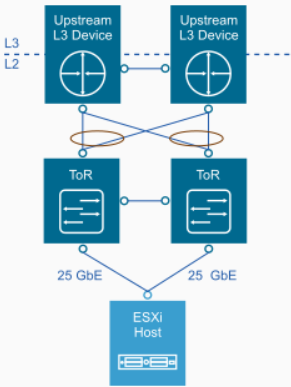
\includegraphics[width=0.5\textwidth]{imaxes/conceptosPrevios/transportlayer2.png}
  \caption{Límite de las capas 2 y 3 cuando la topología se implementa con dispositivos de capa 2.}
  \label{fig:transportlayer2}
\end{figure}
\FloatBarrier
\begin{figure}[h!]
  \centering
  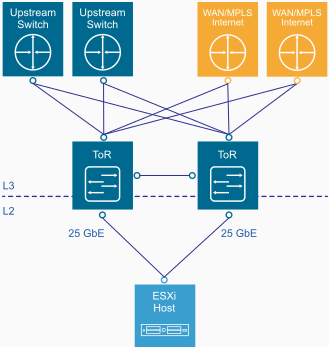
\includegraphics[width=0.5\textwidth]{imaxes/conceptosPrevios/transportNetLayer3.png}
  \caption{Límite de las capas 2 y 3 cuando la topología se implementa con dispositivos de capa 3.}
  \label{fig:transportlayer3}
\end{figure}
\FloatBarrier

\iffalse
n los componentes de VMware, o en la capa tres, para usar dispositivos de transporte lógico. Cada tipo de configuración tiene sus ventajas y desventajas, pero la configuración más común en este tipo de entornos es usar el transporte de red sobre la capa tres ya que da más libertad a la hora de gestionar y configurar los recursos físicos de red.\\
\fi

Como VMware Cloud Foundation abstrae la red física en una red virtual, la red física debe cumplir ciertos requisitos para que la red virtualizada sea robusta. Esta se debe mantener simple con configuraciones comunes en todos los switches, uso de VLANs y uso de enrutamiento dinámico, también debe ser escalable en cuanto a cantidad de hosts, ancho de banda y cantidad de rutas redundantes. Además, se debe tener en cuenta que cada tipo de tráfico tiene características diferentes, como por ejemplo el tráfico dedicado al almacenamiento a través de IP que suele usar mayor ancho de banda, por ello es necesario distinguir cada tipo de tráfico con protocolos QoS. El marcado de cada tipo de tráfico se realiza en el hipervisor ESXi a través de un vSphere Distributed Switch que soporta QoS tanto en la capa 2 como en la capa 3. En la capa 2 se utiliza  un campo de tres bits llamado \textit{Class of Service} que representa la prioridad del \textit{frame} con un valor de cero a siete, presente en la cabecera Ethernet cuando se utiliza etiquetado VLAN, mientras que en la capa 3 se utiliza un campo de 6 bits en la cabecera IP llamado \textit{Differentiated Services Code Point}, perteneciente al protocolo \textit{DiffServ}, para clasificar cada paquete. Los \underline{principales componentes que se deben configurar} para dar conectividad entre los servidores son los siguientes:
\begin{itemize}
    \item \textbf{Top of Rack Physical Switches} (TOR): es un switch al que se conectan los hosts de un rack para tener conectividad con el resto de la infraestructura. Se recomienda que un host esté conectado a dos switches TOR y que estos se configuren de forma redundante para proveer alta disponibilidad y tolerancia a fallos de alguna de las conexiones. Cada switch TOR se conecta a otro par de switches que establece conexión entre todos los racks.
    
    Los puertos del switch TOR que se conectan a los hosts deben estar configurados como puertos troncales de VLAN para que acepte todas las VLANs usadas por el host, se debe proveer servicio DHCP a cada VLAN usada y configurar los puertos para que acepten \textit{jumbo frames}. El marcado QoS del tráfico que realiza cada host ESXi, debe ser aceptado y no puede ser modificado una vez abandona el host. \iffalse Además, se deben configurar todas las VLANs y subredes que se utilizarán en la infraestructura de VMware Cloud Foundation.\fi  
    
    \underline{Otros protocolos que se deben configura}r en los puertos que se conectan con los hosts son:
    \begin{itemize}
        \item \emph{Spanning Tree Protocol} (STP): protocolo que se encarga de gestionar las rutas de la red que son redundantes.
        \item \emph{Trunking}: configurar cada enlace troncal con las VLANs que van a transmitir tráfico a través de él. Se debe establecer como VLAN nativa, aquella utilizada para transmitir el tráfico que no tiene etiqueta, VLAN de la red \textit{management}.
        \item \emph{MTU}: configurar el MTU de cada VLAN para el transporte de paquetes \textit{jumbo frames}. Este valor será el que se use para configurar los hosts ESXi. Se recomienda establecerlo en 9000 bytes.
        \item \emph{Multicast}: configurar el protocolo IGMP en cada switch TOR como enrutador (busca activamente que VLANs pertenecen a un grupo Multicast) y cada VLAN como miembros de IGMP (los hosts que forman parte del grupo indican su pertenencia a un grupo multicast de forma activa).
    \end{itemize}
    

    
    \iffalse
    \item \textbf{Conectividad entre Regiones}: 
    \item \textbf{Conectividad entre Zonas de dispobilidad}:
    \fi
\end{itemize}

\subsubsection{Host ESXi\cite{WDminRequierements}}
Los hosts ESXi que se desplieguen en un cluster deben tener características físicas idénticas para hacer la infraestructura más manejable,  incluyendo la configuración de almacenamiento y red. Para desplegar VMware Cloud Foundation se requiere:
\begin{itemize}
    \item  Dos interfaces de red (NIC) de la misma velocidad que deben estar conectadas a la VLAN troncal de dos switches TOR. Configurando \textit{NIC teaming} en VMware Sphere Distributed Switch se consigue que el tráfico se distribuya por las interfaces de red disponibles de forma óptima y que exista tolerancia a fallos.
    \item Todas las conexiones físicas del host deben tener al menos una velocidad igual a 10 Gbit.
    \item Cada host debe tener al menos 192 GB de memoria RAM, de esa cantidad, 176 GB de memoria RAM son requeridos por las máquinas virtuales que gestionan el SDDC.
    \item Un disco de arranque con un tamaño mínimo de 16 GB.
\end{itemize}

\subsubsection{Almacenamiento físico}
VMware Cloud Foundation utiliza VMware vSAN para proveer el almacenamiento de un SDDC. Para desplegar VMware Cloud Foundation, VMware vSAN requiere las siguientes características:
\begin{itemize}
    \item Mínimo de tres hosts con recursos de almacenamiento.
    \item Determinar qué configuración de vSAN se va a utilizar, \textit{All-Flash} o \textit{Hybrid}. Se recomienda la solución \textit{All-Flash} ya que ofrece mayor rendimiento.
    \item Para cada host con recursos de almacenamiento se debe cumplir que el disco de caché tenga un 10\% de la capacidad del almacenamiento persistente del grupo de discos, tener un mínimo de dos discos en la capa de capacidad, un controlador RAID y configurar habilitar vSphere High Availability  para apagar las máquinas virtuales de un host cuando este se encuentre aislado. El controlador RAID debe tener la característica \textit{pass-through} la cual permite que VMware vSAN muestre como discos individuales cada disco duro de un grupo de discos, esto facilita la gestión de cada disco y que se puedan realizar sustituciones sin detener el servicio.
    \item La capacidad mínima de almacenamiento disponible para el modelo consolidado es de 800 GB. 
\end{itemize}

\end{subsection}



%%%%%DISEÑO ARQ. VIRTUAL
\begin{subsection}{Arquitectura e Infraestructura Virtuales\cite{CFVirtInfraes}}
%%%%%%%%%%%%%%%%%%%%%%%%%%%%%%%%%%%%%%%%%%%%%
%%%%%%%%%%%%%%%%%%%%%%%%%%%%%%%%%%%%%%%%%%%%%
%%%%%%%%%%%%%%%%%%%%%%%%%%%%%%%%%%%%%%%%%%%%%
\iffalse
La infraestructura virtual de un SDDC puede estar formada por una o más regiones, cada una tiene su propio \textit{management domain} que contiene el \textit{management cluster}, y un \textit{virtual infrastructure domain} que contiene el \textit{shared cluster} y un \textit{compute cluster}.
\fi
%%%%%%%%%%%%%%%%%%%%%%%%%%%%%%%%%%%%%%%%%%%%%
%%%%%%%%%%%%%%%%%%%%%%%%%%%%%%%%%%%%%%%%%%%%%
%%%%%%%%%%%%%%%%%%%%%%%%%%%%%%%%%%%%%%%%%%%%%

Esta capa virtual provee infraestructura de almacenamiento, red y cómputo definida por software a través de servicios. En el modelo de despliegue consolidado de VMware Cloud Foundation, todos sus servicios y componentes se encuentran dentro de un mismo cluster (solo una AZ) dentro de la infraestructura, mientras que en el modelo estándar los servicios y componentes de gestión de la infraestructura están situados en clusters distintos (pueden estar en AZ distintintas), todos sus componentes se encuentran agrupados en un mismo cluster.



\subsubsection{VMware vCenter Server}
Este componente es una pieza fundamental dentro del SDDC de VMware. En el modelo consolidado se despliega una instancia de vCenter Server que debe tener conexión con todos los hosts ESXi y con la instancia de Platform Services Controller. Es necesario que exista al menos una instancia de Platform Services Controller en la infraestructura que se puede situar en la misma máquina virtual que vCenter Server o en una máquina virtual dedicada.

%%%%%%%%%%%%%%%%%%%%%%%%%%%%%%%%%%%%%%%%%%%%%%%%%%%%%%%%%%%%%
%%%%%%%%%%%%%%%%%%%%%%%%%%%%%%%%%%%%%%%%%%%%%%%%%%%%%%%%%%%%%
%%%%%%%%%%%%%%%%%%%%%%%%%%%%%%%%%%%%%%%%%%%%%%%%%%%%%%%%%%%%%
\iffalse
Se recomienda desplegar dos instancias, una que administre los componentes que gestionan el SDDC, y otra que administre los servicios \textit{edge} y los \textit{workload domains} de los usuarios, aunque esto depende del uso que se le vaya a dar al SDDC. Además, vCenter Server requiere el despliegue de dos Platform Services Controllers que se pueden colocar dentro de la misma instancia de vCenter Server.
\fi
%%%%%%%%%%%%%%%%%%%%%%%%%%%%%%%%%%%%%%%%%%%%%%%%%%%%%%%%%%%%%
%%%%%%%%%%%%%%%%%%%%%%%%%%%%%%%%%%%%%%%%%%%%%%%%%%%%%%%%%%%%%
%%%%%%%%%%%%%%%%%%%%%%%%%%%%%%%%%%%%%%%%%%%%%%%%%%%%%%%%%%%%%

\subsubsection{Cluster VMware vSphere}
En un SDDC se pueden crear varios clusters vSphere con distintas finalidades, según la cantidad de hosts ESXi, la capacidad de cada uno y del uso que se va a realizar de cada cluster. Además, dentro de la configuración de un cluster hay que considerar como se va a configurar el componente vSphere High Availability para establecer una política de reserva de recursos para restaurar recursos en caso de que un host esté inactivo por algún fallo.\\

En el modelo consolidado se debe crear un único cluster con un mínimo de cuatro hosts ESXi ya que uno de los hosts se utiliza para asegurar la disponibilidad del almacenamiento vSAN cuando hay algún host inactivo. Este modelo proporciona capacidad de un único fallo por cluster.

%%%%%%%%%%%%%%%%%%%%%%%%%%%%%%%%%%%%%%%%%%%%
\subsubsection{Red Virtual}
La red de esta infraestructura está virtualizada por VMware NSX for vSphere. Para un funcionamiento óptimo de la red, se deben seguir las siguientes prácticas en el diseño de las redes virtuales de la infraestructura:
\begin{itemize}
    \item Segmentar los diferentes tipos de tráfico para mejorar la eficiencia de la red y la seguridad. Así se puede ajustar las características de cada red, como el ancho de banda o la latencia, a las necesidades de cada servicio.
    \item Utilizar un único vSphere Distributed Switch por cluster con las distintas redes dedicadas a cada servicio y con diferentes VLANs. La configuración de VLANs debe coincidir con la establecida en la capa física.
    \item Mejorar el rendimiento usando NICs de tipo VMXNET3 en las máquinas virtuales.
    \item Las NICs físicas de cada host ESXi conectadas a un mismo vSphere Distributed Switch deben estar conectadas también a la misma red físicas.
    \item Aquellas redes que se dedican a servicios de la infraestructura deben estar configuradas con puertos tipo \textit{vmkernel}.
\end{itemize}

Para segmentar la red se configura en un vSphere Distributed Switch una VLAN por cada tipo de tráfico que genera VMware vSphere\footnote{Las VLANs descritas se corresponden con el \textit{management} cluster de la arquitectura estándar y con el cluster de la arquitectura consolidada. El resto de clusters del modelo estándar tienen solo las VLANs de los servicios que hay en ellos.}:
    \begin{itemize}
        \item \textbf{Management}: esta VLAN comunica todos los hosts ESXi y por ella se transmite el tráfico enviado entre servicios de VMware Cloud Foundation. Por defecto está configurado en un \textit{vmkernel} con MTU igual a 1500
        \item \textbf{vMotion}: por esta VLAN circula el tráfico del componente vSphere vMotion para realizar las migraciones de máquinas virtuales de un host a otro. Se configura en un \textit{vmkernel} con MTU igual a 9000.
        \item \textbf{vSAN}: a través de esta VLAN los hosts acceden al servicio de almacenamiento mediante dirección IP. Se configura en un \textit{vmkernel} con MTU igual a 9000.
        \item \textbf{VM Network}: por esta VLAN circula el tráfico de las aplicaciones y máquinas virtuales de los usuarios. Se asigna a un \textit{vmportgroup}.
    \end{itemize}
Desde el vSphere Distributed Switch se configuran de forma centralizada todas las VLANs existentes en un cluster. Permite establecer las siguientes características:
\begin{itemize}
    \item \textit{Network I/O Control}: permite establecer un nivel de prioridad a cada VLAN según el servicio que la utiliza sea más o menos crítico. Esto se realiza estableciendo limites de ancho de banda, políticas de balanceo de carga y reserva de recursos para una funcionalidad específica de vSPphere.
    \item \textit{NIC Teaming}: permite aumentar el ancho de banda de la red, balancear la carga del tráfico y reducir el riesgo de fallos. Para poder aplicar esta configuración el host ESXi debe tener conectadas dos NICs al Distributed Switch que físicamente se conectan a dos switches diferentes.
    \item \textit{VXLAN}
\end{itemize}
\begin{figure}[h!]
  \centering
  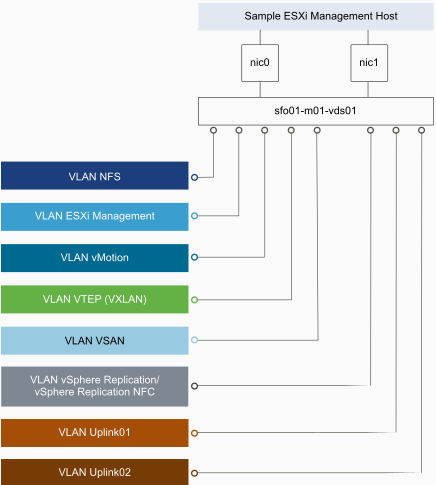
\includegraphics[width=0.65\textwidth]{imaxes/conceptosPrevios/redesVDSCluster.png}
  \caption{Redes virtuales que se utilizan en en la infraestructura para cada componente.}
  \label{fig:redesVirtuales}
\end{figure}
\FloatBarrier



Este utiliza los componentes vCenter Server, NSX Manager, NSX Controllers y NSX Logical Switch para establecer comunicaciones y aislar los distintos tipos de tráfico [Fig. \ref{fig:planosNSX}]. Estos componentes \underline{actúan en diferentes planos} de la red:



\begin{itemize}
    \item \textbf{Plano de Datos}: esta capa gestiona la transmisión del tráfico entre los componentes del SDDC. En este plano actúan NSX Logical Switches segregando los tipos de datos, y el enrutamiento y firewall distribuído de NSX. Se transmite a través de una red física dedicada al transporte.
    \item \textbf{Plano de Control}: aquí se gestionan los mensajes de control que se usan para la configuración de los dispositivos de NSX como switches, routers y firewalls en cada host ESXi. Se distribuye en redes físicas de forma segura usando VLANs para aislarlo del plano de datos.
    \item \textbf{Plano de gestión}: aquí se gestiona el tráfico dedicado a la administración de los recursos como puede ser la creación y eliminación de máquinas virtuales. Está controlado por vCenter Server y NSX Manager.
\end{itemize}
\begin{figure}[h!]
  \centering
  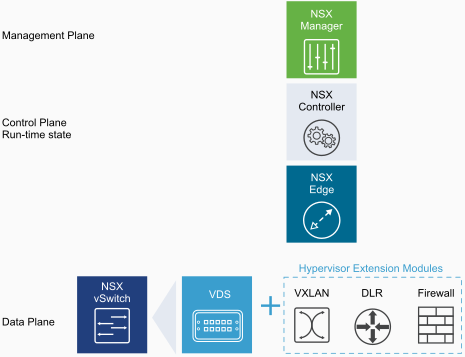
\includegraphics[width=0.65\textwidth]{imaxes/conceptosPrevios/planosNSX.png}
  \caption{Como se estructuran las componentes de VMware NSX for vSphere}
  \label{fig:planosNSX}
\end{figure}
\FloatBarrier
Adicionalmente, VMware NSX incluye diversos servicios que suponen una abstracción lógica de dispositivos físicos de red y que VMware Cloud Foundation utiliza para formar su infraestructura virtual. Estos \underline{servicios son los siguientes}\cite{componentesNSX,nsxCompDesign}:
\begin{itemize}
    \item \textbf{Logical Switches}: permite crear segmentos abstractos que representan dominios de broadcasting donde se colocan determinadas máquinas virtuales. Su tráfico tiene asignado una única VLAN y están mapeados en todos los hosts lo cual simplifica la movilidad de las máquinas virtuales entre los hosts.
    \item \textbf{Universal Distributed Logical Router} (UDLR): realiza las funciones de enrutamiento entre máquinas virtuales y entre \textit{portgroups} de una VXLAN [Pal. \ref{itm:vxlan}]. Se controlan desde una máquina virtual. 
    %y utilizan protocolos de enrutamiento dinámico como BGP y OSPF.
    \item \textbf{Designated Instance}: host ESXi encargado de resolver las solicitudes del protocolo ARP. Es elegido por NSX Controller que escoge un host por cada VLAN existente.
    \item \textbf{Edge Services Gateway} (ESG): también llamado NSX Edge, es el encargado de proveer conectividad a través de la infraestructura física para que los componentes se puedan conectar a redes externas u otras redes del la infraestructura. También aporta firewall de perímetro, balanceo de carga y SSL-VPN.
    \item \textbf{Logical Firewall}: provee mecanismos de seguridad que se asemejan a las funciones de los firewalls físicos pero con la ventaja de que están virtualizados, lo cual hace que su configuración sea más flexible. Trabaja al nivel de puertos \textit{vmkernel} y máquinas virtuales.
    \item \textbf{Logical Load Balancer}: distribuye el tráfico entre los servidores para que el uso de recursos sea el óptimo.
    \item \textbf{VXLAN Tunnel Endpoint} (VTEP): punto donde se encapsula el tráfico de VXLAN en paquetes UDP. Se ubican en los puertos \textit{vmkernel} de un vSphere Distributed Switch.
\end{itemize}



Esta red virtual requiere varios servicios que no están incluídos en VMware Cloud Foundation pero que son necesarios para el correcto funcionamiento del SDDC. Estos \underline{servicios externos} son los siguientes\cite{CFexternalServices}:
\begin{itemize}
    \item \textbf{Servidor DNS}: se utiliza para obtener los nombres y direcciones de todas las máquinas virtuales que se creen, tanto en sentido \textit{fordward} (obtener una dirección IP a partir de un nombre) como en sentido \textit{reverse} (obtener un nombre a partir de una dirección IP). Además, este servicio debe ser configurado antes de realizar el despliegue de VMware Cloud Foundation. Este servicio es utilizado por el componente Platform Services Controller, vCenter Server, NSX Manager y vRealize Log Insight.
    
    \item \textbf{Servidor DHCP}: permite asignar direcciones IP de forma dinámica a los puertos \textit{vmkernel} de cada host ESXi. Este debe ser accesible desde cada VXLAN de VMware NSX y es necesario establecer previamente las redes que se van a usar en VMware Cloud Foundation. Este servicio debe estar disponible antes de comenzar el despliegue del SDDC ya que es necesaria la asignación dinámica de IPs.
    
    \item \textbf{Servidor NTP}: requerido por todos los componentes de VMware Cloud Foundation para mantener sus horas sincronizadas. Este servicio debe estar disponible en la infraestructura y configurado en cada host ESXi antes del despliegue de VMware Cloud Foundation, y debe ser alcanzable desde la red de \textit{management} y de vRealize. La derencia de tiempo entre los componentes de la infraestructura no debe ser mayor de cinco minutos.
    
    \item \textbf{Router}: debe existir enrutamiento dinámico en la red desde la capa 3. Es requerido por NSX para establecer comunicación con los ESG. Este servicio debe estar configurado antes del comenzar enl despliegue de VMware Cloud Foundation. 
\end{itemize}

Respecto a los componentes de gestión de las operaciones que forman parte de la suite VMware vRealize, estos se colocan en una red virtual separada donde solo son accesibles a través de un punto. Esta red contiene una VXLAN que conecta con un UDLR que redirige el tráfico con otras redes a través de los nodos de NSX ESGs. La red entre los nodos de NSX ESGs y el UDLR se demomina red de tránsito [Fig. \ref{fig:vrealizeArch}]. En la figura [\ref{fig:udlrArch}] se puede ver como se estructura el tráfico desde la máquinas virtuales a cada switch TOR usando enrutamiento dinámico.

\begin{figure}[h!]
  \centering
  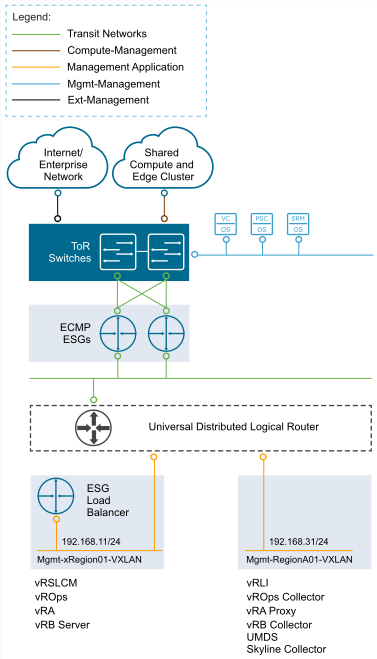
\includegraphics[width=0.6\textwidth]{imaxes/conceptosPrevios/vrealizeARCH.png}
  \caption{Red virtual constuída para alojar los componentes de VMweare vRealize.}
  \label{fig:vrealizeArch}
\end{figure}
\begin{figure}[h!]
  \centering
  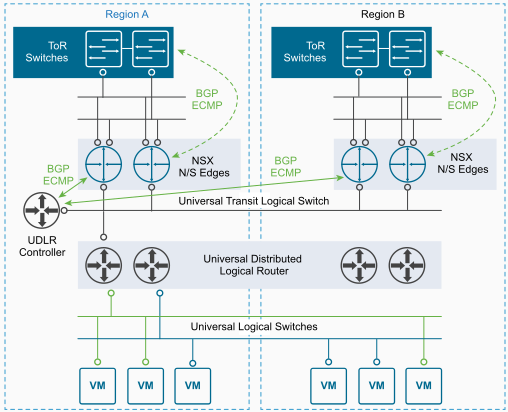
\includegraphics[width=0.6\textwidth]{imaxes/conceptosPrevios/UDLRroutingNSX.png}
  \caption{Arquitectura del enrutamiento dinámico de NSX.}
  \label{fig:udlrArch}
\end{figure}
\FloatBarrier


\subsubsection{Almacenamiento Virtual}
VMware vSAN forma único \textit{datastore} con todos los dispositivos de almacenamiento que se encuentran en la infraestructura permitiendo establecer políticas y gestionar esos recursos de forma más simple. Para que funcione correctamente es necesario \underline{configurar una red para VMware vSAN} teniendo en cuenta los siguientes aspectos:
\begin{itemize}
    \item El uso de vSpehere Distributed Switches genera mejor rendimiento.
    \item Se recomienda el uso de paquetes tipo \textit{jumbo frames}.
    \item Asignar una VLAN al tráfico de cada cluster de VMware vSAN.
    \item Si se implementa en un SDDC con dos localizaciones, es necesario establecer un host \textit{witness}.
\end{itemize}
Al establecer el tamaño y capacidad de este cluster hay que tener en cuenta que cuantos más hosts ESXi se incluyan, mayor tolerancia a fallos se tendrá y mejor se podrán repartir los grupos de discos entre todos los hosts. Debe haber un balance entre el hardware y la capacidad requerida.
\end{subsection}


\begin{subsection}{Operaciones de la Arquitectura\cite{CFopermanagement}}
En este apartado se define como se gestionan en VMware Cloud Foundation las tareas de administración de todas las partes de la infraestructura. Estas tareas se agrupan en la gestión del ciclo de vida y la recopilación de información sobre el estado de cada componente existente.

\subsubsection{Gestión del Ciclo de Vida}
Elementos que se encargan de administrar el ciclo de vida de los componentes:
\begin{itemize}
    \item \textbf{vSphere Update Manager}: pensado para la adminstración del entorno vSphere. Permite administrar las actualizaciones del software de virtualización, instalar software de terceros en los hosts ESXi y actualizar el hardware virtual de las máquinas virtuales. Existe una instancia de este producto por cada instancia de vCenter Server y se puede elegir entre dos modelos de despliegue, uno en el que se usa una máquina virtual denominada \textbf{Update Manager Download Service} (UMDS) que se encarga de descargar los archivos requeridos por vSphere Update Manager mientras este se encuentra en un entorno aislado [Fig. \ref{fig:updateManager}], y otro donde es la instancia de vSphere Update Manager la que realiza la descarga de los ficheros. La primera opción incrementa la seguridad y permite compartir estos archivos entre distintas instancias de vSphere Update Manager.\\
    Una vez desplegado se pueden establecer diferentes configuraciones a nivel de host, máquina virtual y cluster, para que durante la instalación de actualizaciones el servicio del SDDC continúe operativo y evitar la pérdida de información y errores en los recursos.
    
    \item \textbf{vRealize Suite Licfecycle Manager}: elemento encargado de administrar el ciclo de vida de todos los productos de vRealize de forma automatizada, esto incluye el despliegue, configuración, instalación de actualizaciones y escalamiento de los productos vRealize Operations Manager, vRealize Log Insgiht y vRealize Automation. Este se conecta a un servicio externo para descargar los archivos que se necesiten [Fig. \ref{fig:vrealizeUpdateManager}]. Se despliega como una máquina virtual y una sola instancia se encarga de gestionar los productos de varias regiones en caso de que las haya.

\end{itemize}

\begin{figure}[h!]
  \centering
  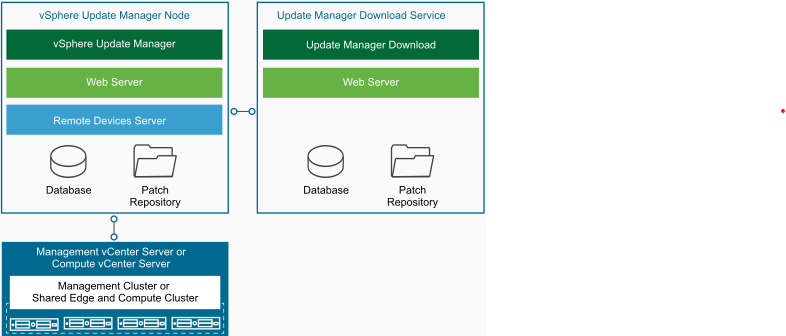
\includegraphics[width=0.8\textwidth]{imaxes/conceptosPrevios/vSphereUpdate.png}
  \caption{Estructura de la gestión del ciclo de vida con vSphere Update Manager.}
  \label{fig:updateManager}
\end{figure}
\begin{figure}[h!]
  \centering
  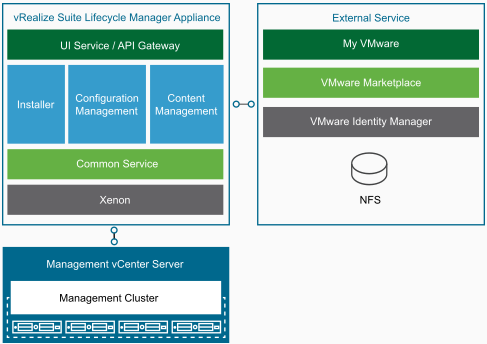
\includegraphics[width=0.8\textwidth]{imaxes/conceptosPrevios/vRealizeUpdateArchLifeCyle.png}
  \caption{Estructura de la gestión del ciclo de vida con vRealize Suite Lifecycle Manager.}
  \label{fig:vrealizeUpdateManager}
\end{figure}
\FloatBarrier

\subsubsection{Gestión de Logs}
En VMware Cloud Foundation el producto vRealize Log Insight provee gestión y análisis de los logs de la infraestructura. Este componente conecta con los componentes Platform Services Controller, vCenter Server, hosts ESXi, todos los componentes de NSX y todos los productos de la suite de VMware vRealize para recoger la información que generan sobre alarmas, tareas y eventos que tienen lugar usando el protocolo Syslog.\\
vRealize Log Insight está formado por un nodo \textit{Master} y dos nodos \textit{Worker}. Esto permite proveer alta disponibilidad al habilitar el balanceador de carga \textit{Integrated Load Balancer} (ILB), quien se encarga de recibir las peticiones de logs de los clientes y luego las retransmite a los nodos \textit{worker} y \textit{master} para obtener la información. Inicialmente se despliegan con la configuración reducida.
%El segundo modo consiste en desplegar único nodo \textit{Master} que realiza las funciones de un nodo \textit{Master} y un nodo \textit{Worker}. Inicialmente


Estos nodos se sitúan en una red diferente a al resto de componentes situados en la red \textit{management} de VMware vSphere, a los cuales acceden mediante un Universal Distributed Logical Router y enrutamiento dinámico BGP [Fig. \ref{fig:vrealizeArch}].

\end{subsection}
